\documentclass[tikz,border=8pt]{standalone}
\usepackage[T1]{fontenc}
\IfFileExists{libertine.sty}{\usepackage{libertine}}{}
\IfFileExists{inconsolata.sty}{\usepackage[scaled=0.94]{inconsolata}}{}
\usetikzlibrary{arrows.meta,calc}

\definecolor{ink}{RGB}{38,45,53}
\definecolor{muted}{RGB}{111,120,129}
\definecolor{rulegray}{RGB}{210,216,222}
\definecolor{softgray}{RGB}{247,248,249}
\definecolor{structure}{RGB}{39,91,144}
\definecolor{structurefill}{RGB}{241,246,251}
\definecolor{metadata}{RGB}{181,109,25}
\definecolor{metadatafill}{RGB}{253,248,239}

\begin{document}
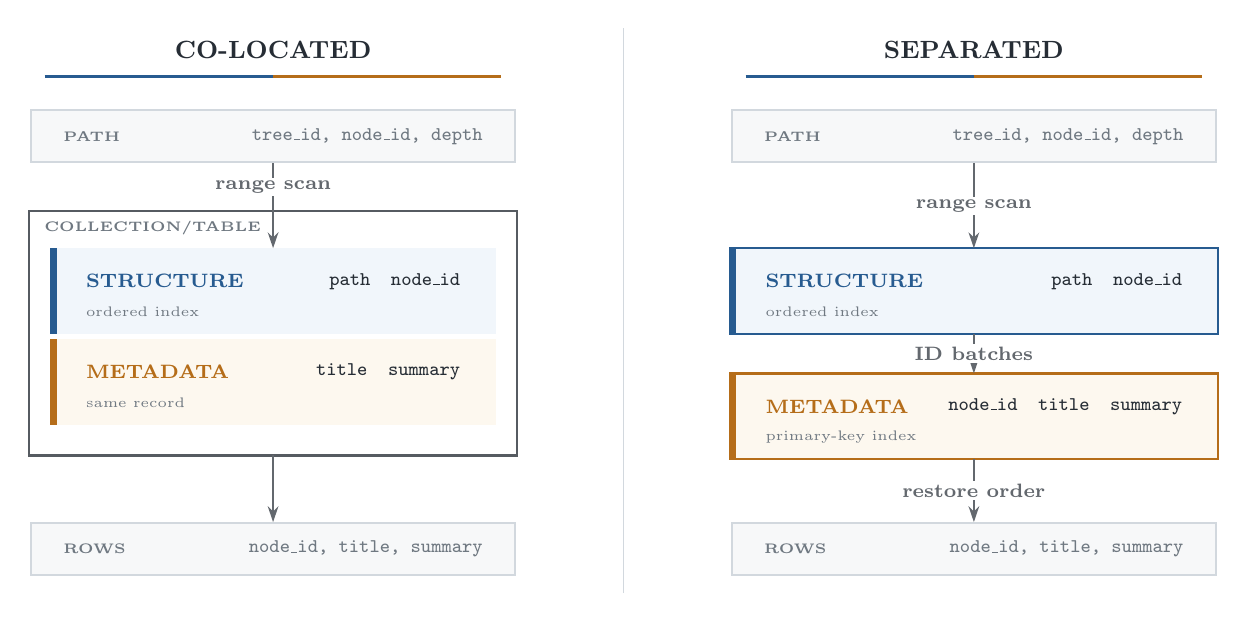
\begin{tikzpicture}[
  x=1cm,y=1cm,
  font=\sffamily,
  flow/.style={-{Stealth[length=2.0mm,width=1.35mm]}, draw=ink!72,
               line width=0.8pt},
  action/.style={font=\scriptsize\bfseries, text=ink!72, fill=white,
                 inner xsep=2.4pt, inner ysep=1pt},
  field/.style={font=\scriptsize\ttfamily, text=ink},
  endpoint/.style={draw=rulegray, fill=softgray, line width=0.65pt,
                   minimum width=6.15cm, minimum height=0.66cm}
]

% Headings and a single quiet divider keep the comparison on one visual plane.
\node[font=\small\bfseries, text=ink] at (4.05,7.25) {CO-LOCATED};
\draw[structure, line width=1.15pt] (1.15,6.91) -- (4.05,6.91);
\draw[metadata, line width=1.15pt] (4.05,6.91) -- (6.95,6.91);

\node[font=\small\bfseries, text=ink] at (12.95,7.25) {SEPARATED};
\draw[structure, line width=1.15pt] (10.05,6.91) -- (12.95,6.91);
\draw[metadata, line width=1.15pt] (12.95,6.91) -- (15.85,6.91);

\draw[rulegray, line width=0.6pt] (8.50,0.35) -- (8.50,7.52);

% Identical inputs.
\node[endpoint] (pathL) at (4.05,6.15) {};
\node[anchor=west, font=\tiny\bfseries, text=muted]
  at ([xshift=3mm]pathL.west) {PATH};
\node[anchor=east, font=\scriptsize\ttfamily, text=muted]
  at ([xshift=-3mm]pathL.east) {tree\_id, node\_id, depth};

\node[endpoint] (pathR) at (12.95,6.15) {};
\node[anchor=west, font=\tiny\bfseries, text=muted]
  at ([xshift=3mm]pathR.west) {PATH};
\node[anchor=east, font=\scriptsize\ttfamily, text=muted]
  at ([xshift=-3mm]pathR.east) {tree\_id, node\_id, depth};

% Co-located layout. The shared outline is the collection/table boundary.
\draw[ink!78, line width=0.95pt] (0.95,2.10) rectangle (7.15,5.20);
\node[anchor=west, font=\tiny\bfseries, text=muted]
  at (1.02,4.98) {COLLECTION/TABLE};

\fill[structurefill] (1.22,3.64) rectangle (6.88,4.73);
\fill[structure] (1.22,3.64) rectangle (1.30,4.73);
\node[anchor=west, font=\scriptsize\bfseries, text=structure]
  at (1.55,4.31) {STRUCTURE};
\node[anchor=east, field] at (6.55,4.31) {path\quad node\_id};
\node[anchor=west, font=\tiny, text=muted]
  at (1.55,3.92) {ordered index};

\fill[metadatafill] (1.22,2.49) rectangle (6.88,3.58);
\fill[metadata] (1.22,2.49) rectangle (1.30,3.58);
\node[anchor=west, font=\scriptsize\bfseries, text=metadata]
  at (1.55,3.16) {METADATA};
\node[anchor=east, field] at (6.55,3.16) {title\quad summary};
\node[anchor=west, font=\tiny, text=muted]
  at (1.55,2.77) {same record};

\draw[flow] (pathL.south) -- (4.05,4.73)
  node[action, pos=0.28] {range scan};

% Separated layout. Structure and metadata have independent boundaries.
\draw[structure, line width=0.9pt, fill=structurefill]
  (9.85,3.64) rectangle (16.05,4.73);
\fill[structure] (9.85,3.64) rectangle (9.93,4.73);
\node[anchor=west, font=\scriptsize\bfseries, text=structure]
  at (10.18,4.31) {STRUCTURE};
\node[anchor=east, field] at (15.72,4.31) {path\quad node\_id};
\node[anchor=west, font=\tiny, text=muted]
  at (10.18,3.92) {ordered index};

\draw[metadata, line width=0.9pt, fill=metadatafill]
  (9.85,2.05) rectangle (16.05,3.14);
\fill[metadata] (9.85,2.05) rectangle (9.93,3.14);
\node[anchor=west, font=\scriptsize\bfseries, text=metadata]
  at (10.18,2.72) {METADATA};
\node[anchor=east, field] at (15.72,2.72)
  {node\_id\quad title\quad summary};
\node[anchor=west, font=\tiny, text=muted]
  at (10.18,2.33) {primary-key index};

\draw[flow] (pathR.south) -- (12.95,4.73)
  node[action, midway] {range scan};
\draw[flow] (12.95,3.64) -- (12.95,3.14)
  node[action, midway] {ID batches};

% Identical ordered outputs.
\node[endpoint] (rowsL) at (4.05,0.91) {};
\node[anchor=west, font=\tiny\bfseries, text=muted]
  at ([xshift=3mm]rowsL.west) {ROWS};
\node[anchor=east, font=\scriptsize\ttfamily, text=muted]
  at ([xshift=-3mm]rowsL.east) {node\_id, title, summary};

\node[endpoint] (rowsR) at (12.95,0.91) {};
\node[anchor=west, font=\tiny\bfseries, text=muted]
  at ([xshift=3mm]rowsR.west) {ROWS};
\node[anchor=east, font=\scriptsize\ttfamily, text=muted]
  at ([xshift=-3mm]rowsR.east) {node\_id, title, summary};

\draw[flow] (4.05,2.10) -- (rowsL.north);
\draw[flow] (12.95,2.05) -- (rowsR.north)
  node[action, midway] {restore order};

\end{tikzpicture}
\end{document}
